\documentclass[conference]{IEEEtran}
\IEEEoverridecommandlockouts
% The preceding line is only needed to identify funding in the first footnote. If that is unneeded, please comment it out.
\usepackage{cite}
\usepackage{amsmath,amssymb,amsfonts}
\usepackage{algorithmic}
\usepackage{graphicx}
\usepackage{textcomp}
\usepackage{xcolor}
\def\BibTeX{{\rm B\kern-.05em{\sc i\kern-.025em b}\kern-.08em
    T\kern-.1667em\lower.7ex\hbox{E}\kern-.125emX}}
\begin{document}

\title{Implementation of convolutional neural networks to classify mammograms from a breast cancer cohort.}

\author{\IEEEauthorblockN{Cesar Sanchez-Villalobos}
\IEEEauthorblockA{\textit{Department of Electrical and Computer Engineering} \\
\textit{Texas Tech University}\\
Lubbock, TX \\
cesarasa@ttu.edu}
\and
\IEEEauthorblockN{Fernando Koiti Tsurukawa}
\IEEEauthorblockA{\textit{Department of Electrical and Computer Engineering} \\
\textit{Texas Tech University}\\
Lubbock, TX \\
fetsuruk@ttu.edu}
}

\maketitle

\begin{abstract}
According to both NIH and the RSNA, Breast Cancer (BC), is the most common type of cancer diagnosed to women in the United States. One of the methods currently used in radiology to diagnose BC, is the mammography screening, where an mammogram is taken from the patient and then a trained physician needs to look into patterns and check if the patient could be diseased. In order to reduce the costs of the mammography screening, it is of high interest use Deep Learning (DL) algorithms to aid the decision making. The following document serves as a report for the final assignment of the Data Science class, where we analyzed a dataset and implemented Convolutional Neural Networks (CNNs) to classify the mammograms into either Control, or diseased. 
\end{abstract}

\begin{IEEEkeywords}
Breast Cancer, Deep Learning, Convolutional Neural Networks, Data Analysis, Image Processing
\end{IEEEkeywords}

\section{Introduction}

The following document is a report for our final project during the Data Science class, delivered by Dr. Mary Baker at Texas Tech University. During the project, we joined a kaggle competition named \textit{RSNA Screening Mammography Breast Cancer Detection}. During this competition, the Radiological Society of North America (RSNA), provided a dataset of both control and BC patients with their mammograms to promote the research of DL techniques in their field. 

Therefore, we did a brief data analysis, the implementation of data balancing techniques and several CNNs to perform the classification task. Therefore, the following document is divided as follows: first, we have a discussion about our data analysis and the data provided by RSNA. Second, we discuss the problems of data leakage and data imbalance, which are the most common problems in DL and the reproducibility of results. Third, we discuss the methods used for solving these problems and to train the neural networks. In chapter IV, we present our results and finally, we give a brief discussion in the conclusion. 

\section{RSNA Breast Cancer Dataset}

The RSNA dataset is an anonymized dataset publicly released by RSNA as a designed experiment to aid the identification of cancer cases using mammogram screening. This dataset has both the metadata and the mammograms for each patient, in the metadata, we have access to the following information:

\begin{itemize}
\item Source hospital: it is an ID number to know where the images were taken. 
\item ID of the patient: each patient has an assigned number. 
\item ID of the image: as each patient has several images, it is necessary to know which image are we looking. 
\item Laterality: each patient has at least two images of the right breast, and two images of the left breast. 
\item Mammography view: all the patients have a least two views of each breast. In a usual screening, we take two classic types of images, the mediolateral oblique (MLO) view, and the cranial caudal view. 
\item Implant: we need to know if there are artifacts inside the images, this might be an issue for any implementation.
\item Density: a phenotypic trait of the breast. 
\item Biopsy: some screenings lead to biopsy. In this column we have which one went for a biopsy. 
\item Invasive: a phenotypic trait of some of the tumors. 
\item BIRADS: a rating of how likely is for the patient have cancer. There are several NaNs in this column. 
\item Age: the age of the patient at the moment of the screening. 
\item Cancer: our target, this is a binary column where the ones are positive values, and the zeros are healthy controls.
\end{itemize}



\subsection{Types of view in a mammogram screening:}

In both the challenge overview and the literature review, we can see that in most mammogram screenings the physician takes two views of each breast, the mediolateral oblique (MLO) and the cranial caudal (CC) views. According to Mohamed et al, the CC view is taken from above the breast and the MLO view is taken from one side of the breast, aligning the center of the chest and imaging outwards. These two views are not the only available views in the whole dataset, but they are the views that we are interested in, as most of the patients only have these two images. 

In Figure \ref{fig:types_of_view}, we can see the most common types of views according to Mohamed et al, using images from the RSNA dataset. Note that for this patient, we will have an extremely dark image, as the volume of the breast is not spread over all the taken image. Note also that there are annotations with the view on the corners of the images. 

\begin{figure}[ht]
\centering
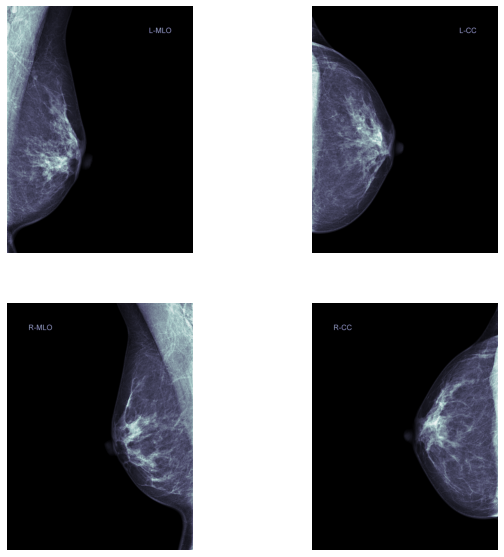
\includegraphics[width=3.2in]{breast_images}
\caption{Example of the views for one patient. In the left column we can see the MLO view, and in the right column we can see the CC view. }
\label{fig:types_of_view}
\end{figure}

\subsection{Exploratory Data Analysis}

The RSNA data has a total of 11913 different patients, where 11427 are healthy control subjects and 486 are Breast Cancer subjects. Note that in this case we have a heavily imbalanced problem, as it is usually the case for biomedical imaging problems. The data has records of six different types of views including MLO and CC, and each patient indeed has at least 4 images. A distribution of patients per number of images, is shown in Figure \ref{fig:image_dist}. 

\begin{figure}[ht]
\centering
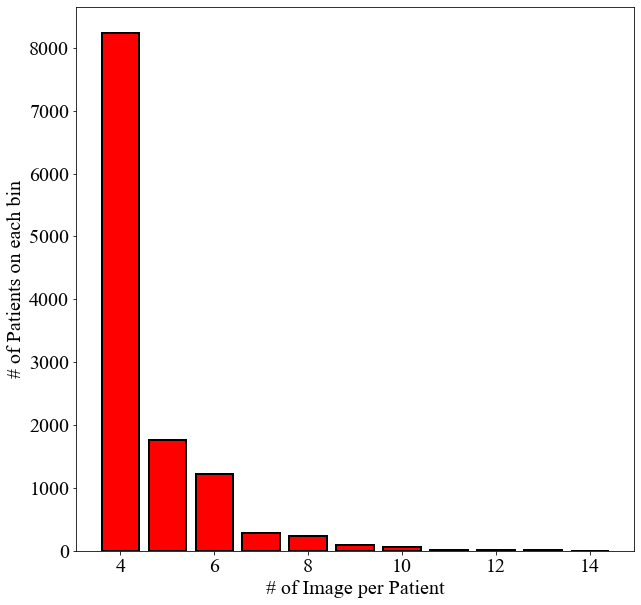
\includegraphics[width=3in]{images_dist}
\caption{Distribution of patients per number of Images.}
\label{fig:image_dist}
\end{figure}

Note that over 8000 of the patients have only 4 images (the CC and MLO views for their two breasts), and only a small number of patients have more than 6 images. All these images sum to a total of 54706 images, where 53548 are labeled as Non-Cancer images and 1158 as showing cancer. It is important to note that from these 53548 images, we also have 1477 that are showing an implant. These implant may be targeted as problematic when we are training, so it is important to highlight that they could be an issue in any screening. Finally, a distribution of the ages of the patients is shown in Figure \ref{fig:ages}.


\begin{figure}[ht]
\centering
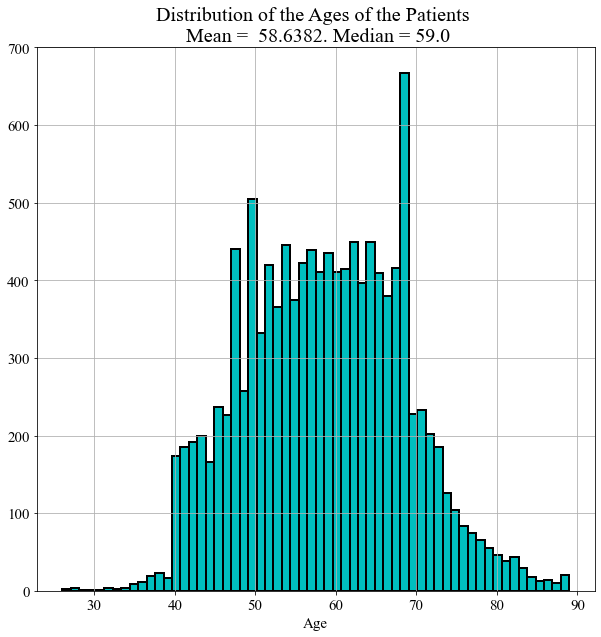
\includegraphics[width=3in]{age_distributions}
\caption{Age Distribution. }
\label{fig:ages}
\end{figure}

Note that we have low representations of ages before 40 years. This is mainly due to the idea that a risk factor of breast cancer in women is being over 40 years old. Then, the distribution shows a heavy tail on the left and a normal tail on the right. This suggests that the data is slightly skewed, the computed skewnes was $0.103$, the Kurtosis was $-0.354$, the youngest patient was 26 years old, whereas the oldest was 89. The mean and the median are also visible in Figure \ref{fig:ages}. 

\section{Problems to Solve}

While we studied the RSNA dataset with our exploratory data analysis (EDA), we detected three critical problems to solve before the DL implementation. These problems were Data Imbalance, Data Leakage, and the hetereogenity of the images. In this section we will define these problems. 

\subsection{Data Imbalance}

In the context of machine learning and statistics, we refer to \textit{class imbalance} to the event where there are more observations of one class, than the other available classes in the dataset. This is specially detrimental when we train any kind of DL model, as it leads to a poor performance when we try to predict the underrepresented class. 

Data imbalance is a problem in machine learning as it could lead to models that are biased towards the majority class. This is because the model is more likely to learn from the majority class data, and will therefore be more likely to predict the majority class.

In our case, a 96\% of our data is labeled as healthy. This represents a heavily imbalanced classification problem, as setting a classifier that always points into the healthy label, will give a 96\% of accuracy but 0 recall. The goal then, would be to improve the 0 recall into a more suitable number. 

There are four ways to solve this issue in our case: 

\begin{itemize}
\item \textbf{Undersampling the majority class:} the designer of the experiment can sample without replacement from observations in the majority class. This can be done until the number of samples per class is the same. 

\item \textbf{Oversampling the minority class:} the designer of the experiment can sample with replacement from observations in the minority class. This can be done until the number of samples per class is the same. However, a drawback of this method is that with a heavily imbalanced class, we will end up with all the instances repeated, which might be also detrimental to the problem.

\item \textbf{Data augmentation of the minority class:} the designer of the experiment can sample with replacement from observations in the minority class, however, to each sampled instance, a random transformation will be applied to it. The transformation can include one or several types of: geometric transformation, probabilistic transformations, non linear transformation, including additive or multiplicative random noise, among others. This will ensure to have different instances and a suitable number of data points, which is desirable for Deep Learning problems. 

\item \textbf{Generative methods: } with images, in the past two years we have seen the increase of generative approaches for images like DALL-E and Stable Diffusion, and more classical methods like the Generative Adversarial Networks (GANs). All of these methods end up creating synthetic images, and synthesizing patterns to create new images from the minority class, would be a potential solution for the Data Imbalance problem. 
\end{itemize}

\subsection{Data Leakage}

We refer to data leakage as the event where some information used in the training stage of the model, will appear in the evaluation stage. In this case, we have to be very careful when we split our dataset into train and test sets, as if we do it image-wise, we will end up with images from the same patient in both sets. Therefore, to solve this issue, we will be splitting the dataset patient-wise. 

\subsection{Image related issues}

As the images are coming from different hospitals and, sometimes, from different imaging machines, they present different sizes and contrasts. Also, the dataset is large, it has a size of 116 GB of information and all the images are stored in DICOM format.  

The DICOM format, is highly used in clinical environments as it allows the physician to store metadata related to the patient and the machine. As we will only need the pixel array, we will just save the arrays into JPEG format to save space. 

\section{Methods and Preprocessing}

\subsection{Image Processing}

VOI LUT
ROI methods
Undersampling 
\subsection{Convolutional Neural Network}

\section{Results}
\subsection{Baseline Model}
blah blah
\subsection{Model with extracted ROIs}
worse 
\subsection{Extra models (this might be tricky given the timeline, as we don't have results)}
let's pray
\section{Conclusion and Suggestions}



\end{document}
